%
% Although we try to provide a template that completely
% matches the corresponding assignment, we do expect you
% to check that you have indeed answered all questions.
%

% ALSO VERY IMPORTANT:
% This is just a template to help you with the LaTeX part of the assignment.
% So you may change it completely according to your own wishes!
%

\documentclass[a4paper]{article}
% Typically the 'article' class is appropriate for assignments.
% And we print it on a4, so we include that as well.

\usepackage{a4wide}
% To decrease the margins and allow more text on a page.

\usepackage{graphicx}
% To deal with including pictures.

\usepackage{enumerate}
% To provide a little bit more functionality than with LaTeX's default
% enumerate environment.

\usepackage{array}
% To provide a little bit more functionality than with LaTeX's default
% array environment.

\usepackage[american]{babel}
% Use this if you want to write the document in US English. It takes care of
% (usually) proper hyphenation.
% If you want to write your answers in Dutch, please replace 'american'
% by 'dutch'.
% Note that after a change it may be that the first compilation of LaTeX
% fails. That is normal and caused by the fact that in auxiliary files
% from previous runs, there may still be a \selectlanguage{american}
% around, which is invalid if 'american' is not incorporated with babel.

\usepackage{amssymb}
% This package loads mathematical things like the fonts for the blackboard
% bold for the set of natural numbers.

\usepackage{tikz}
\usetikzlibrary{arrows}
\usepackage{array}
% The tikz package can be used to draw all kinds of diagrams.
% In this assignment it is being used for drawing the parse trees.

\usepackage[all]{xy}
% Instead of tikz you can also use xy to draw parse trees with

% Some obscure definition to create a circled node within xy.
% The definition is made by Freek Wiedijk who prefers to do his definitions
% in TeX instead of LaTeX, which explains the \def instead of \newcommand.
\def\node{*++[o][F-]}
\def\fnode{*++[o][F=]}

\newcommand{\exercise}[2]{\subsection*{Exercise #1}{#2}}
\newcommand{\exerciseenum}[2]{\subsection*{Exercise #1}{\begin{enumerate}[a)]#2\end{enumerate}}}
% We defined our own commands to make it easy to present all the
% exercises in the same style. The first one does not automatically
% start an 'enumerate' list, the second one does.
% The [2] means that our command needs two arguments.
% The #1 and the #2 indicate where we use these arguments in the
% command.
% There are several ways to have automatic numbering for the exercises,
% but here we have chosen to use a subsection for this and use manual
% numbering. This is because maybe not everyone will be able to do hand in
% all exercises.
% Note that we add the '*' to make sure that the subsection is not numbered.
% (Since we don't have a \section, the numbers for a subsection would be
% ugly like 0.1, 0.2 et cetera.
% The environment 'enumerate' automatically numbers the items in this list.
% The optional [a)] makes sure that the list will be like a), b), c) et cetera.



\newcommand{\abs}[1]{\ensuremath{\left|\, #1 \,\right|}}
\newcommand{\floor}[1]{\ensuremath{\left\lfloor\, #1 \,\right\rfloor}}
\newcommand{\ceil}[1]{\ensuremath{\left\lceil\, #1 \,\right\rceil}}
% Abbreviations for the absolute value, ceil and floor function.

\newcommand{\set}[1]{\ensuremath{\left\{{#1}\right\}}}
% This command puts curly braces around its argument, so it becomes
% a set. The \left and \right make sure that the braces grow in size
% if the contents of the set are large symbols.

\newcommand{\setbuild}[2]{\ensuremath{\set{{#1}\mid{#2}}}}
% We also introduce a shortcut for using the set builder notation.
% Do you understand what it does?

\newcommand{\seq}[1]{\ensuremath{\left\{{#1}\right\}}}
% This puts curly braces to define a sequence.
% Note that this is the same as the definition for a \set.

% And the next series of commands gives you some of the default sets
% that were in the slides.
\newcommand{\TT}{\ensuremath{\mathbb{T}}}
\newcommand{\FF}{\ensuremath{\mathbb{F}}}
\newcommand{\NN}{\ensuremath{\mathbb{N}}}
\newcommand{\NNp}{\ensuremath{\mathbb{N}^{+}}}
\newcommand{\ZZ}{\ensuremath{\mathbb{Z}}}
\newcommand{\ZZp}{\ensuremath{\mathbb{Z}^{+}}}
\newcommand{\QQ}{\ensuremath{\mathbb{Q}}}
\newcommand{\QQp}{\ensuremath{\mathbb{Q}^{+}}}
\newcommand{\RR}{\ensuremath{\mathbb{R}}}
\newcommand{\RRp}{\ensuremath{\mathbb{R}^{+}}}
\newcommand{\CC}{\ensuremath{\mathbb{C}}}

% An the next command gives a shorthand for the power set of a given set.
\newcommand{\power}[1]{\ensuremath{{\cal P}\left({#1}\right)}}

% Below is the tikz-definition that is used for the parse trees.
\tikzset{
  treenode/.style = {
    align=center,
    inner sep=0pt,
    text centered,
    font=\sffamily},
  arn_n/.style = {
    thick,
    treenode,
    circle,
    font=\sffamily\bfseries,
    draw=black,
    %text width=1.5em,
    minimum size=1.5em
    },
  arn_r/.style = {
    treenode,
    circle,
    red,
    draw=red,
    %text width=1.5em,
    minimum size=1.5em,
    very thick},
}

\title{Mathematical Structures\\Assignment 3}

% Replace the placeholders by your real name, student number and
% group (for the exercise hours)
\author{Tony Lopar \\ s1013792 \quad Group 1}

% In LaTeX everything before \begin{document} is called pre-amble.
% This is where you put all important settings. The real document
% starts after \begin{document}.
\begin{document}
\maketitle
% \maketitle makes sure that the title is shown on the first page of
% the document.


% Now we use the command we defined earlier and give it the proper two
% parameters.
% Because the second parameter is long, we put a % directly after the
% opening curly brace {. This is not needed but makes the source file
% look a bit better.
\exerciseenum{19}{%
\addtocounter{enumi}{2}
\item%c
The formula
$p \to  q$
can be represented by the sentence
`If I bought a lottery ticket this week, then I won the million dollar jackpot'.
%In LaTeX opening quotes should be made with ` and closing quotes with '
\addtocounter{enumi}{4}
\item%h
The formula
$\neg p \lor  (p \land  q)$
can be represented by the sentence
`I didn't bought a lottery ticket this week or I bought a lottery ticket and won the million dollar jackpot'.
}

\exerciseenum{20}{%
\addtocounter{enumi}{1}
\item%b
The sentence
`You get an A on the final, you do every exercise in this
book, and you get an A in this class.'
can be represented by the formula
\[p \land q \land r\]
\addtocounter{enumi}{2}
\item%e
The sentence
`Getting an A on the final and doing every exercise in
this book is sufficient for getting an A in this class.'
can be represented by the formula
\[(p \land q) \to r\]
}

\exerciseenum{21}{%
\addtocounter{enumi}{2}
\item%c
The biconditional
`$1 + 1 = 3$ if and only if monkeys can fly.'
is true, because both statements are false, so the truth value of the proposition will be true.
}

\exerciseenum{22}{%
\addtocounter{enumi}{2}
\item%c
The `or' in the sentence
`To enter the country you need a passport or a voter
registration card.'
is an `inclusive or',
because you will probably not be refused at the border when you have both of them.
}

\exerciseenum{23}{%
\item%a
The parse tree for the formula
$p\to\neg p$
is:
% Obviously this is not the correct tree, but it might give you an idea
% how to create the proper one.
\begin{center}
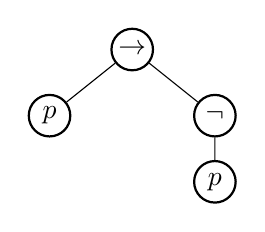
\begin{tikzpicture}[-,
  >=stealth',
  level/.style={
    sibling distance = 3cm, % This parameter can be used to place the nodes
                            % further apart horizontally.
    level distance = 1.2cm}, % This parameter can be used to place the nodes
                             % further apart vertically.
  scale=0.7]
\node [arn_n] {$\to$} % We start with the root (operator)
    % The arn_n is specified to use a specific set that is defined above in
    % \tikzset.
    % This root operator is binary so it has two children.
    child { node [arn_n] {$p$} % First child of the root.
          }
    child { node [arn_n] {$\neg$} % Second child of the root.
            % This second child of the root has again two children.
            child { node [arn_n] {$p$} % First child on second level.
                  }
          }
;
\end{tikzpicture}
\end{center}

\addtocounter{enumi}{1}
\item%c
The parse tree for the formula
$q \lor p  \lor\neg s  \lor\neg r  \lor\neg t \lor u$\
is:
\begin{center}
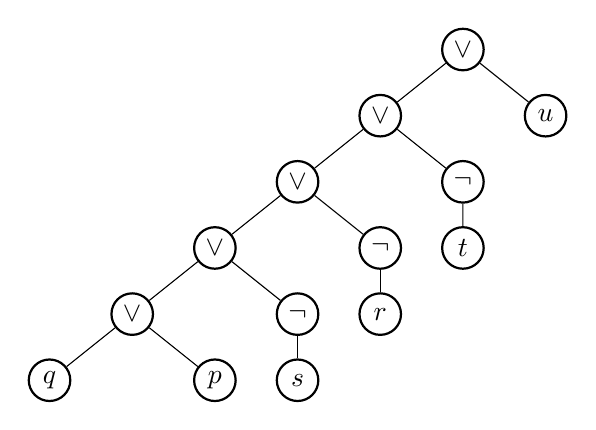
\begin{tikzpicture}[-,
  >=stealth',
  level/.style={
    sibling distance = 3cm, % This parameter can be used to place the nodes
                            % further apart horizontally.
    level distance = 1.2cm}, % This parameter can be used to place the nodes
                             % further apart vertically.
  scale=0.7]
\node [arn_n] {$\lor$} % We start with the root (operator)
    % The arn_n is specified to use a specific set that is defined above in
    % \tikzset.
    % This root operator is binary so it has two children.
    child { node [arn_n] {$\lor$} % First child of the root.
            child { node [arn_n] {$\lor$} % Second child of the root.
                child { node [arn_n] {$\lor$} % Third child of the root.
                    child { node [arn_n] {$\lor$} % 4th child of the root.
                        child { node [arn_n] {$q$} % 5th child of the root.
                        }
                        child { node [arn_n] {$p$} % 5th child of the root.
                        }
                    }
                    child { node [arn_n] {$\neg$} % 4th child of the root.
                        child { node [arn_n] {$s$} % 5th child of the root.
                        }
                    }
                }
                child { node [arn_n] {$\neg$} % Third child of the root.
                    child { node [arn_n] {$r$} % 4th child of the root.
                    }
                }
            }
            child { node [arn_n] {$\neg$} % Second child of the root.
                child { node [arn_n] {$t$} % Third child of the root.
                }
            }
          }
    child { node [arn_n] {$u$} % First child of the root.
          }
;
\end{tikzpicture}
\end{center}
%\end{center}
% In xymatrix you place the nodes manually as in a matrix.
% Columns are separated by & and the end of the row is given by \\
% Not that if you only have empty columns you can immediately the \\
% When you have put the nodes on their place, you add the arrows,
% starting from each node.
% The [dr] indicates an arrow that goes one down and one to the right in
% the matrix. Read the manual if you want to see how you can draw
% all kinds of other arrows.

}

\exercise{24}{%
We have to show that
$(p  \lor \neg q) \land (q  \lor \neg r)\land  (r  \lor \neg p)$
is true when $p$, $q$, and $r$ have the
same truth value and it is false otherwise.

\begin{enumerate}[i)]
\item
We start by assuming that $p$, $q$ and $r$ have the same truth value.
In every part of the proposition then will be two different values, since the negation value of another atomic proposition will have the opposite truth value. This means that in every part of the proposition there will be a atomic proposition with truth value T and the other will have F. The disjunction will make all propositions true. So the proposition will have 3 values T connected by a conjunction which will have the truth value true.
\item
And now we assume that $p$, $q$ and $r$ do not all have the same truth value.
Let's assume that the truth value of p will be F and the truth values of q and r will be true. In this case $(p \lor \neg q)$ will result false, because both atomic propositions are false. So one of the truth values in the conjunction will be false, which makes the proposition false. If we assumed that p is true and another atomic proposition would be false, then $(q \lor \neg r)$ or $r \lor \neg p$ would be false, which would also make the truth value of the proposition false.
\end{enumerate}
}

\exerciseenum{25}{%
\addtocounter{enumi}{1}
\item%b
The negation of the sentence
`Carlos will bicycle or run tomorrow.'
is Carlos will not run and will not bike tomorrow
}

\exerciseenum{26}{%
\addtocounter{enumi}{4}
\item%e
The formula
$\neg(p\to  q)\to p$
is a tautology.
We prove this without using truth tables.

\smallskip
When a proposition is a tautology this means that it should be always true. Let us assume that
the formula would not be a tautology, then at least one of the truth values has to be false. The proposition can only be false when $\neg (p \to q)$ is true and $p$ is false. If we eliminate the negation then $(p \to q)$ needs to have the truth value false. We know that $p$ has to be false, but the proposition $p \to q$ will be true when p is false, no matter the value of q. This means the whole proposition cannot have a false truth value, so it's a tautology.
}

\exerciseenum{27}{%
\item%a
The statement
$a \land b \vDash a$
is true,
because in order for this proposition to be false $a \land b$ needs to be true and $a$ false. If a is false, then the proposition $(a \land b)$ will also be false, because of the conjunction. This means the proposition cannot be false which means it's a tautology.
\addtocounter{enumi}{1}
\item%c
The statement
$\vDash a \lor  (b \to a)$
is false,
because the proposition will be false when $a$ and $(b \to a)$ both have the truth value false. If we take $a = true$ and $b = false$, then $b \to a$ will be false and since $a$ is also false the proposition will be false. This means the proposition cannot be a tautology.
\addtocounter{enumi}{2}
\item%f
The statement
$a \land \neg a \vDash b$
is true,
because the proposition $(a \land \neg a)$ will always be false, since there will always be a true and a false in the conjunction. In order for the proposition to be false, $b$ should be false and $(a \land \neg a)$ should be true. Since $(a \land \neg a)$ is always false the whole proposition cannot be false, which means that the proposition is a tautology.
}

\exerciseenum{28}{%
    \item Show that $(p \to r) \lor (q \to r)$ and $(p \land q) \to r$ are logically equivalent.
    \newline
    In order for two propositions to be logically equivalent they should have exactly the same truth value for every value of p and q. In the truth table we can see that the values of both propositions(marked green) are equal for all inputs of the atomic propositions p and q. The biconditional statement of these two propositions will always result true.

    \begin{tabular}{c|c|c|c|c|c|c|c}
        $p$ & $q$ & $r$ & $p \to r$ & $q \to r$ & $(p \to r)\lor (q \to r)$ & $p \land q$ & $(p \land q)\to r$\\
        \hline
        T & T & T & T & T & {\color{green} T} & T & {\color{green} T}\\
        T & T & F & F & F & {\color{green} F} & T & {\color{green} F}\\
        T & F & T & T & T & {\color{green} T} & F & {\color{green} T}\\
        T & F & F & F & T & {\color{green} T} & F & {\color{green} T}\\
        F & T & T & T & T & {\color{green} T} & F & {\color{green} T}\\
        F & T & F & T & F & {\color{green} T} & F & {\color{green} T}\\
        F & F & T & T & T & {\color{green} T} & F & {\color{green} T}\\
        F & F & F & T & T & {\color{green} T} & F & {\color{green} T}\\
    \end{tabular}
}


\end{document}
